\chapter{Исследовательская часть}

В данном разделе будут приведены примеры работы программ, постановка эксперимента и сравнительный анализ алгоритмов на основе полученных данных.

\section{Технические характеристики}

Технические характеристики устройства, на котором выполнялись замеры времени, следующие:

\begin{itemize}
	\item операционная система: Arch Linux;
	\item память: 48 Гб;
	\item процессор: AMD Ryzen 7 3700X 8-Core Processor (16 ядер);
	\item видеокарта: Nvidia GeForce GTX 1080 (8 Гб, 2560 Cuda ядер, 20 SM по 128 Cuda ядер).
\end{itemize}

\section{Демонстрация работы программы}

Ниже представлены некоторые примеры работы программы.
Продемонстрирована работа виртуальной геометрии.

\begin{figure}[ph!]
	\centering
	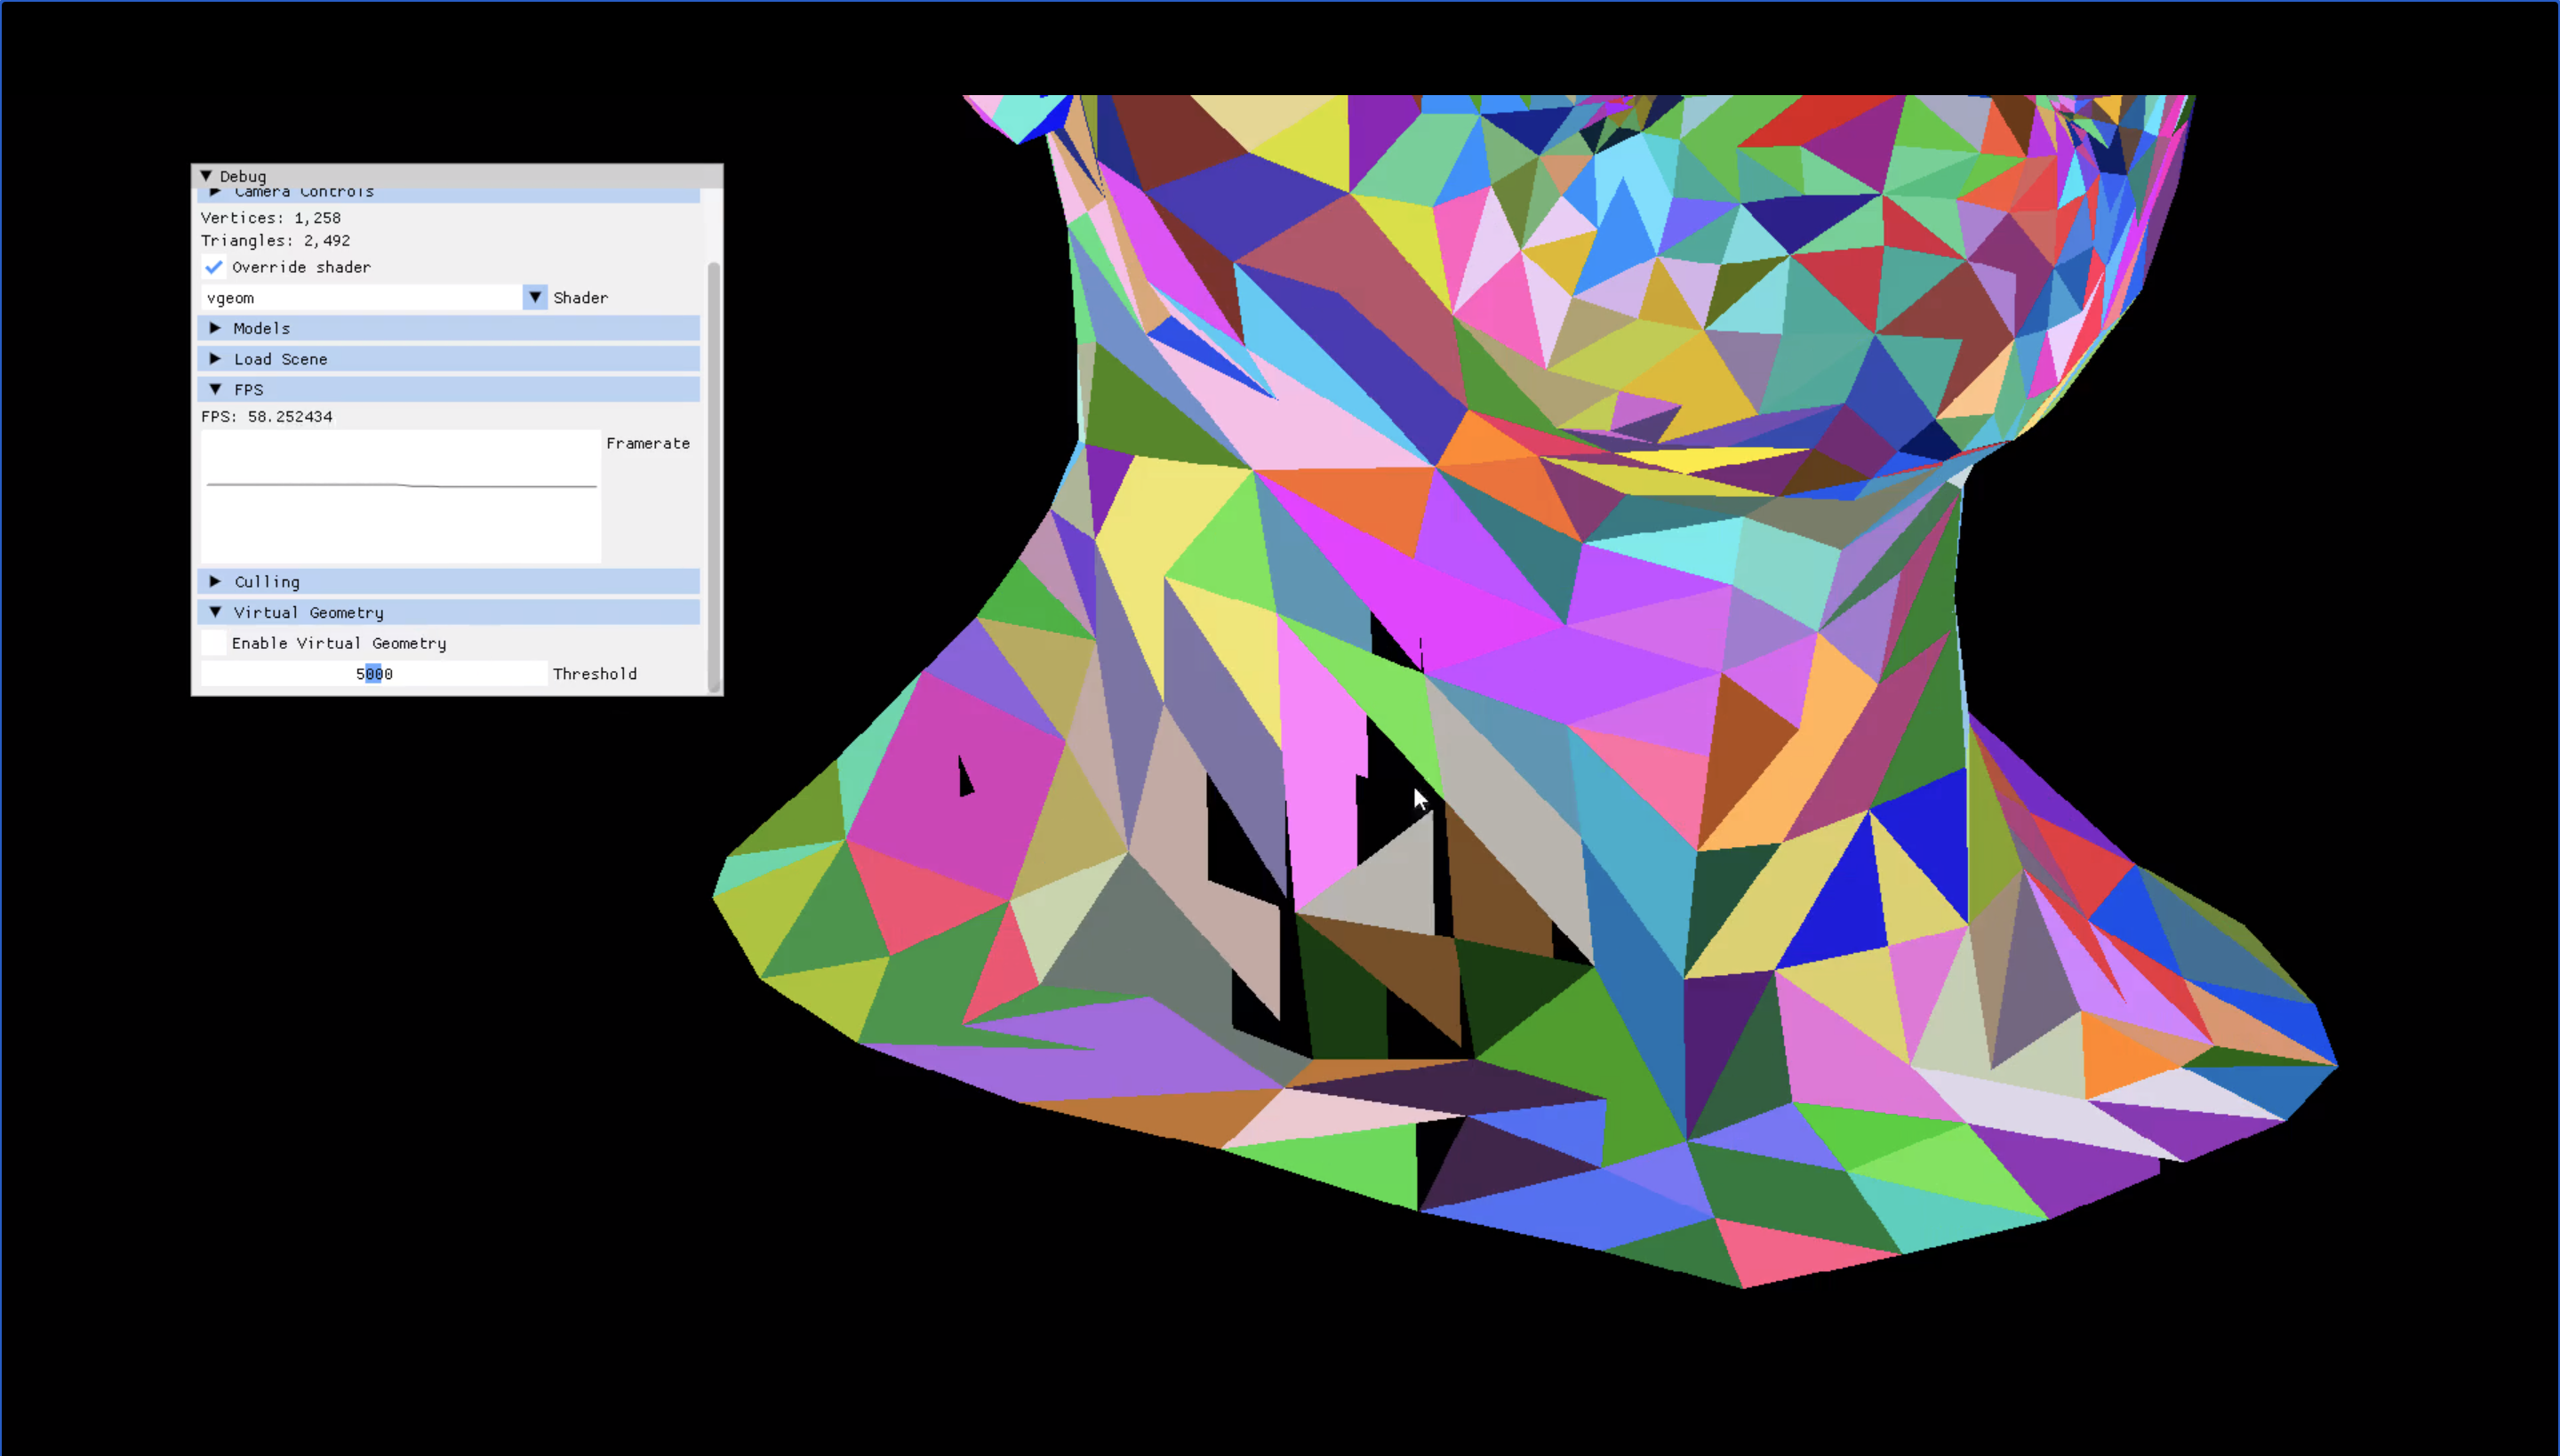
\includegraphics[width=0.95\linewidth]{inc/img/vgeom_off.png}
	\caption{Геометрия объекта сцены с отключенной виртуальной геометрией. FPS=30.}
\end{figure}

\begin{figure}[ph!]
	\centering
	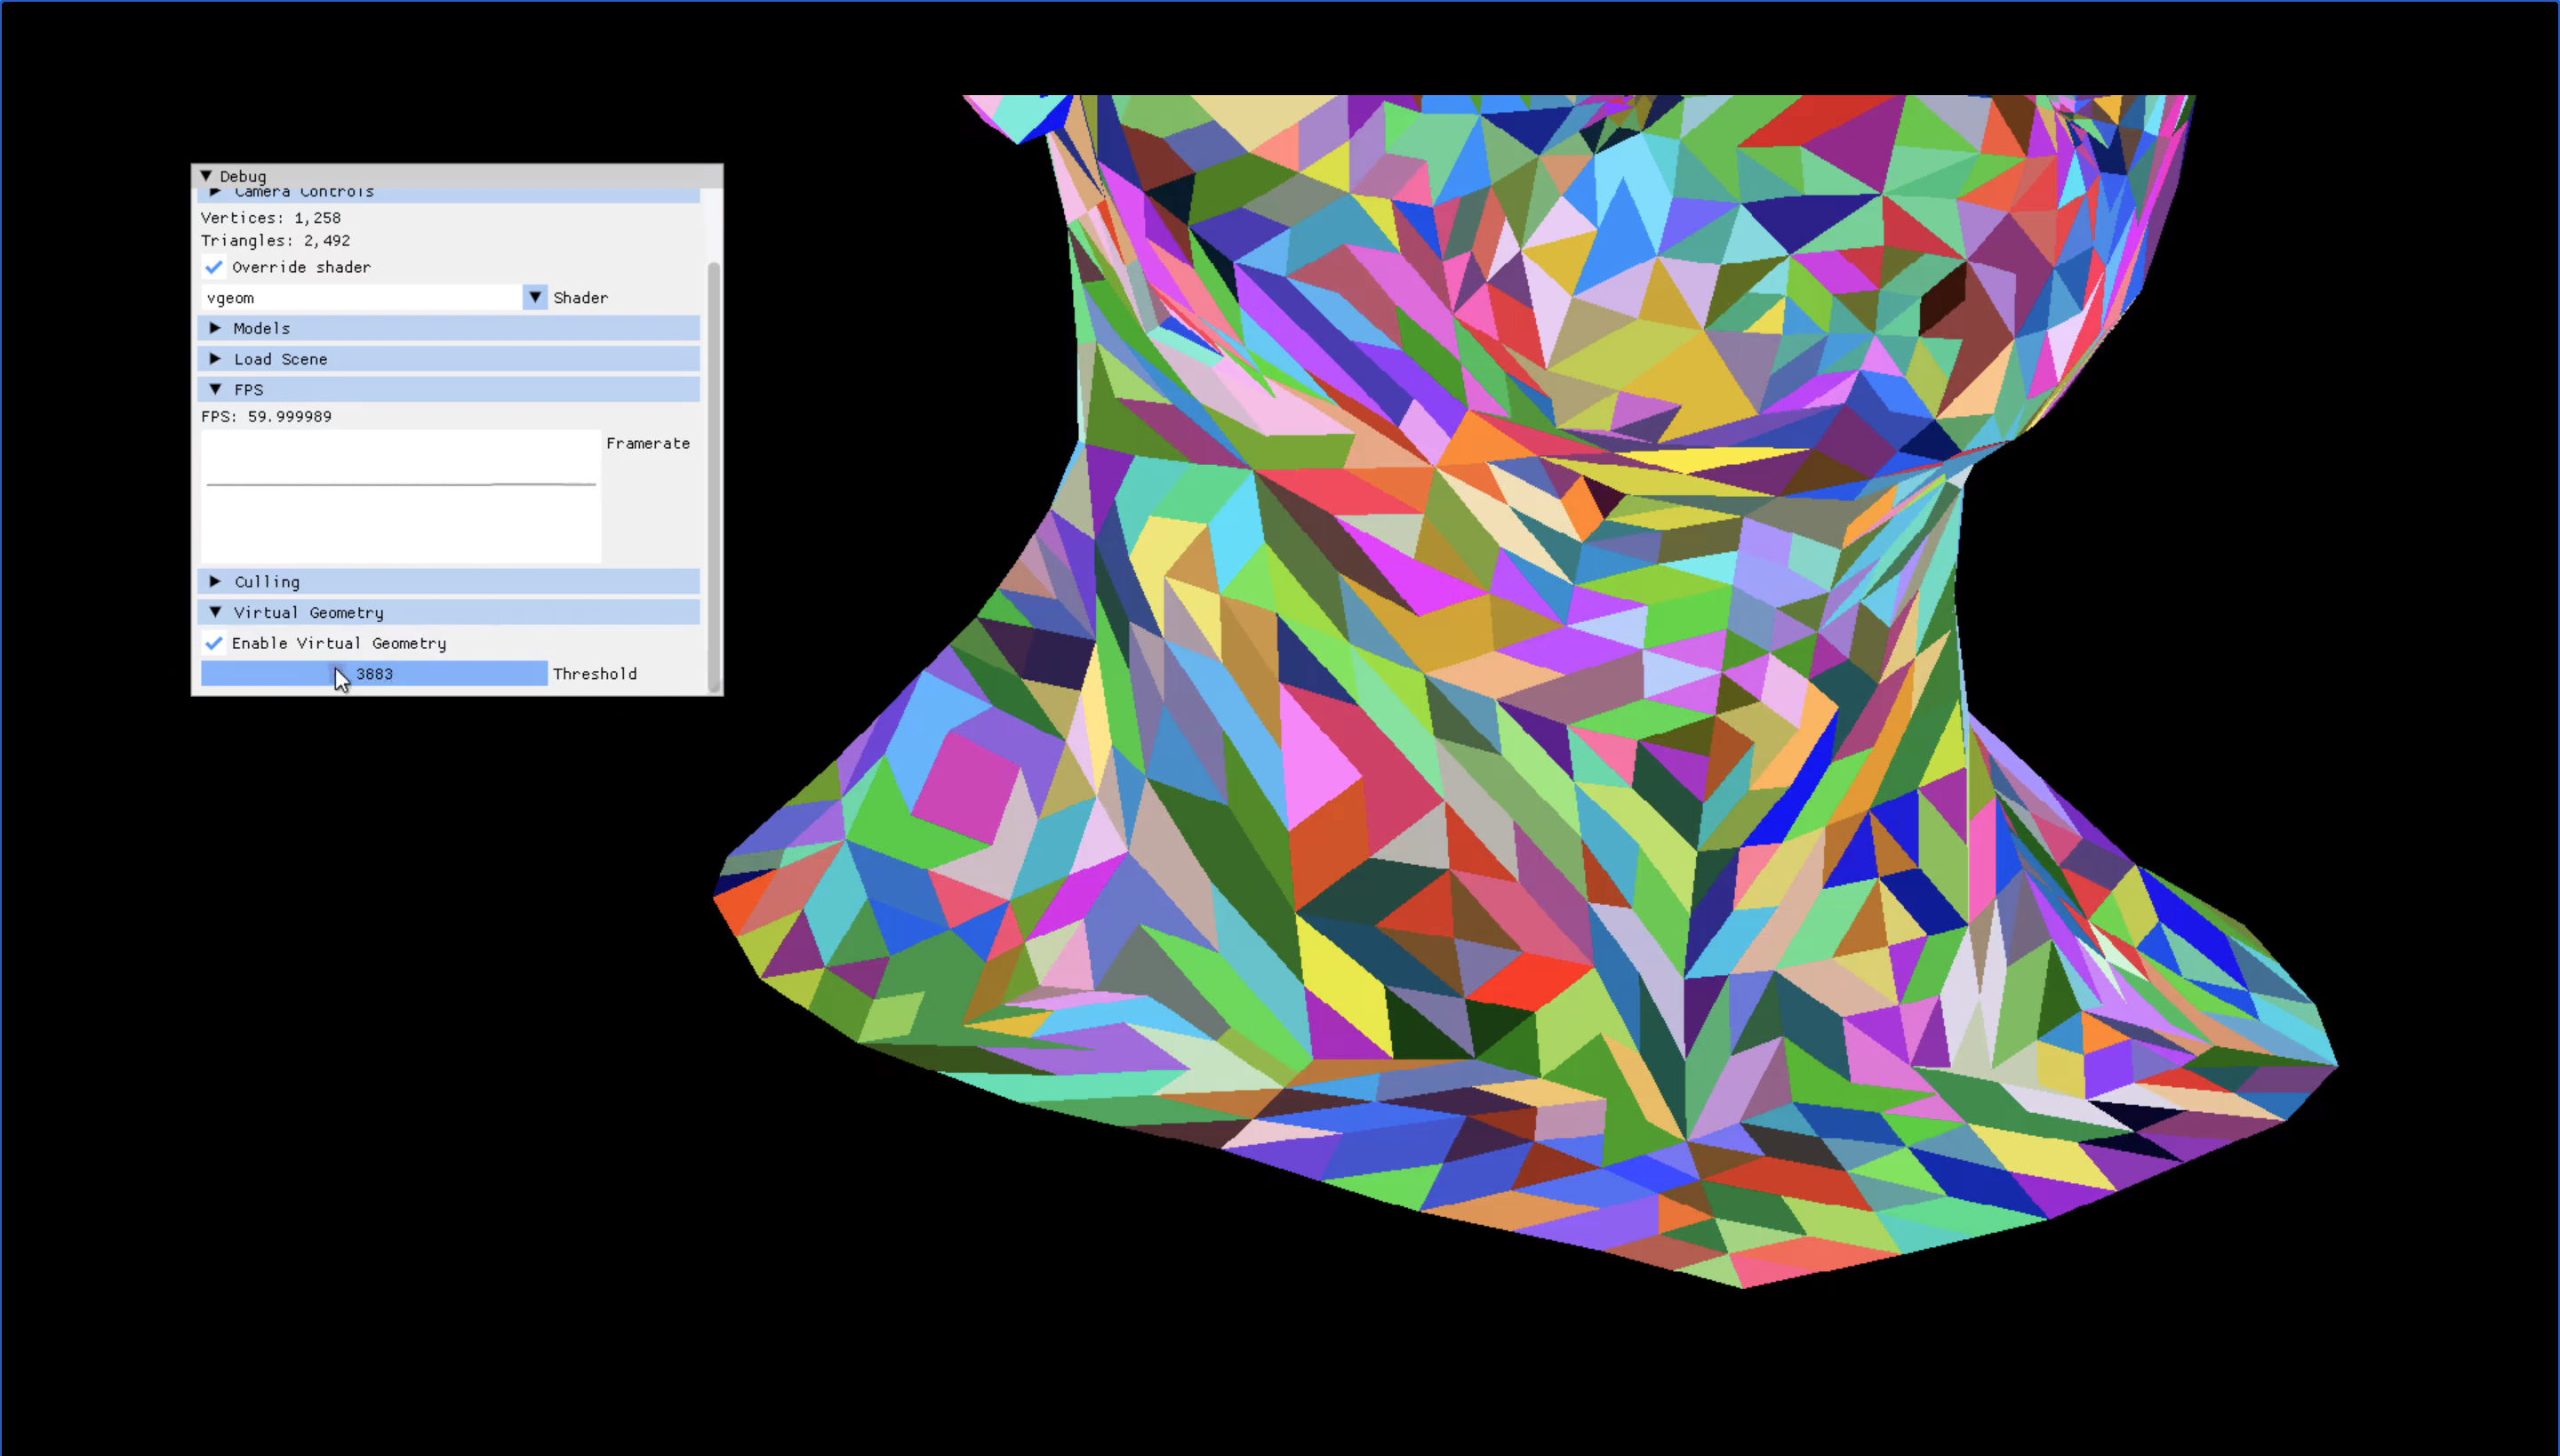
\includegraphics[width=0.95\linewidth]{inc/img/vgeom_on.png}
	\caption{Геометрия объекта сцены с включенной виртуальной геометрией. FPS=60.}
\end{figure}

\pagebreak

\subsection{Замеры FPS в зависимости от количества потоков} 

Замер FPS проводился на сцене с 1000 объектами, с выключенной виртуальной геометрией и включенным куллингом.
Отрисовывалось порядка 1500 объектов. Видно что при увеличении количества потоков FPS растет, но не линейно.
Во время разработки, количество потоков в блоке полагалось равным 32. При этом FPS был равен 30. 
При использовании 6 потоков, FPS оставался примерно таким же, как и при 32 потоках. Этот результат оказался неожиданным. Можно сказать, что 
API CUDA сам диспетчеризует задачи, игнорируя количество потоков в блоке. 
При использовании 1 потока, FPS был равен 8. Результат ожидаем.

\begin{figure}[ph!]
	\centering
	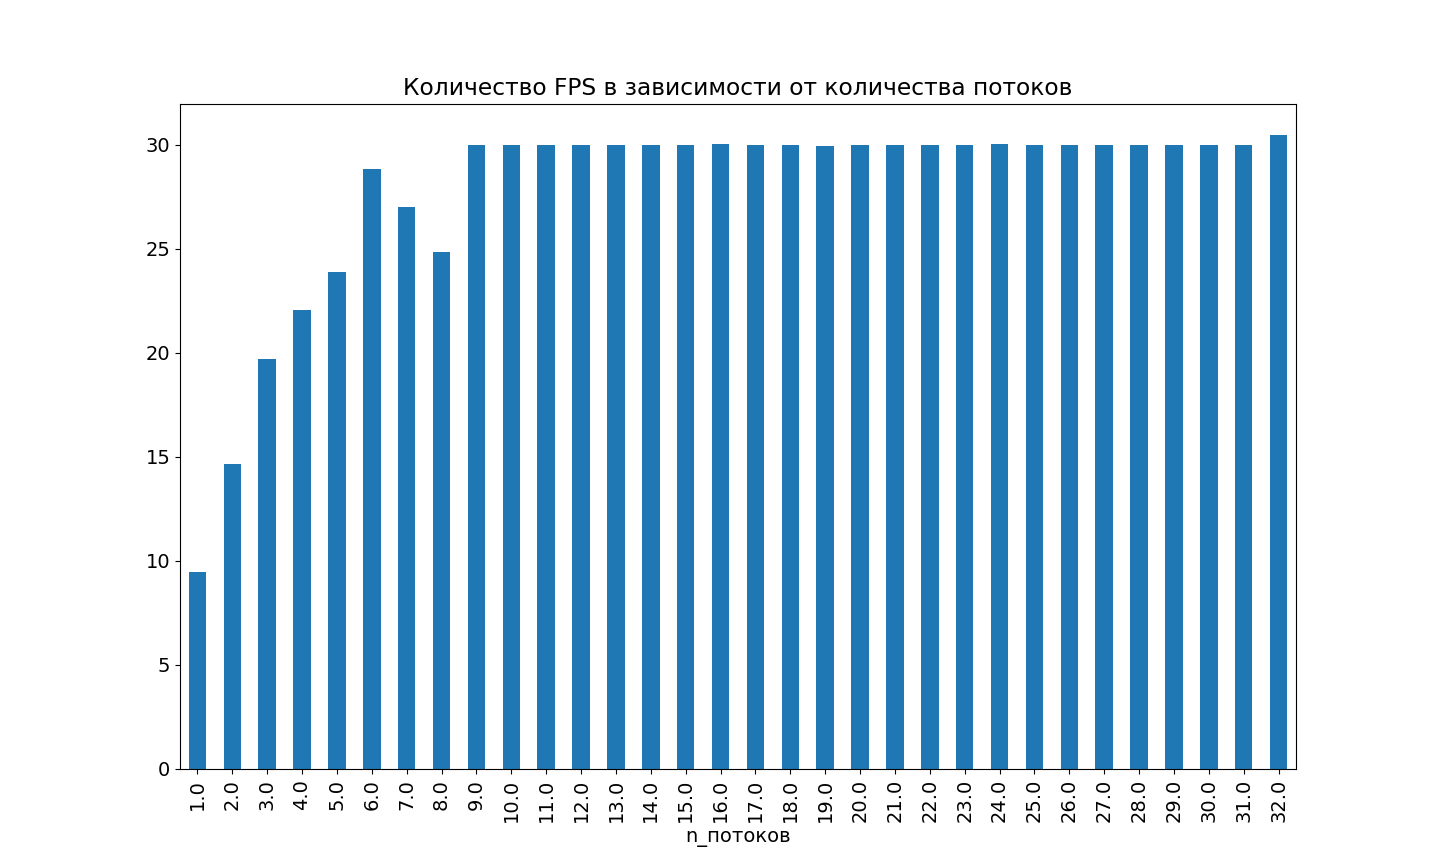
\includegraphics[width=0.95\linewidth]{inc/img/fps_per_threads_2.png}
	\caption{Среднее значение FPS в зависимости от количества потоков в блоке.}
\end{figure}

%\begin{figure}[ph!]
%	\centering
%	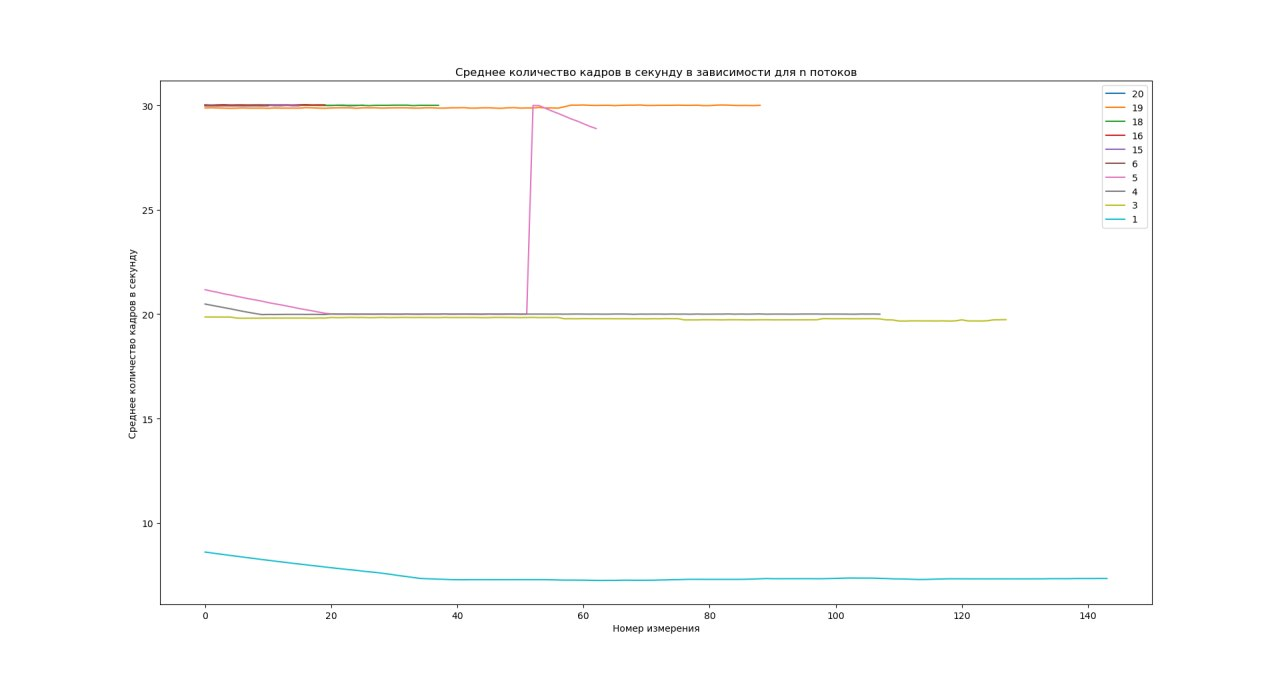
\includegraphics[width=0.95\linewidth]{inc/img/fps_for_threads.jpg}
%	\caption{Значения FPS в зависимости для разного количества потоков в блоке.}
%\end{figure}

\pagebreak

\begin{table}[ph!]
	\centering
	\begin{center}
		\begin{threeparttable}
		\caption{Зависимость FPS от количества потоков. }
		\label{tbl:random}
			\centering
			\begin{tabular}{|l|l|}
				\toprule
				 N потоков &   fps \\
				\midrule
						1 &  8.109443 \\
						3 & 19.825833 \\
						4 & 20.685212 \\
						5 & 22.320932 \\
						6 & 29.966984 \\
					   14 & 29.996874 \\
					   15 & 29.981960 \\
					   16 & 30.018676 \\
					   18 & 29.998919 \\
					   19 & 29.901213 \\
					   20 & 29.998437 \\
					   24 & 30.015810 \\
					   25 & 29.989560 \\
					   32 & 30.018723 \\
				\bottomrule
				\end{tabular}
		\end{threeparttable}
	\end{center}
\end{table}

\pagebreak

\section*{Вывод}

Использование массивно параллельной архитектуры SIMT видеокарты позволило существенно ускорить процесс программной растеризации.
Производительность уступает графическим API (Vulkan, OpenGL), но не такая плохая, как ожидалось.
Можно говорить о выполнении растеризации в реальном времени (во всех тестах количество кадров в секунду было больше 24).
Проведены замеры количества кадров в секунду в зависимости от количества потоков в блоке.
Даны обоснования полученным результатам.
